\RequirePackage{lineno}
\documentclass[11pt,draft]{article}
\usepackage[final]{graphicx}
\usepackage{ucs,multicol,natbib,ifdraft,mathtools,xfrac,float,hyperref}
\usepackage[utf8x]{inputenc}
\usepackage[T1]{fontenc}
\usepackage[romanian]{babel}
\usepackage[a4paper,margin=2cm]{geometry}
\usepackage[printonlyused,withpage]{acronym}
\usepackage[usenames]{color}
\usepackage[obeyDraft,colorinlistoftodos]{todonotes}

\floatstyle{boxed}
\restylefloat{figure}
\setlength{\columnsep}{25pt}

\graphicspath{ {./img/} }
\DeclareGraphicsExtensions{.pdf,.png,.jpg}

\presetkeys{todonotes}{inline}{}

\bibpunct{(}{)}{;}{a}{,}{,}
 
\makeatletter
\def\closeopenmulticols{%
   \def\@tempa{multicols}%
   \ifx\@tempa\@currenvir
      \end{multicols}%
  \fi 
}

\makeatother
\newcommand\Section[1]{%
 \closeopenmulticols
  \begin{multicols}{2}[\section{#1}]
}


% close last open multicols
\AtEndDocument{ \closeopenmulticols}

\title{Studiu observațional asupra tratamentului incontinenței urinare de efort la pacientele din ambulator}
\author{Dr.~Andrei~Manu-Marin,~medic~primar~urologie\\Gnosis-EvoMed, str.~Suvenir,~nr.~10,~sect.~2,~București}
\date{\todo{data studiu}}

\begin{document}

\maketitle\ifdraft{\linenumbers}{ }\todototoc\listoftodos

\begin{abstract}
\ac{IU} este definită ca orice pierdere involuntară a urinei. \ac{IU} face parte din categoria de simptome ale tractului urinar inferior (prescurtare: \ac{LUTS}) care includ dificultăți atât legate de stocarea urinei cât și de eliminarea ei, \ac{IU} fiind în categoria simptome de
stocare. \ac{IU} poate fi caracterizată în plus prin datele obținute în urma anamnezei și a contextului simptomelor descrise de pacient. \todo{Mai multe detalii despre studiu}
\end{abstract}
  
\Section{Introducere}
\ac{IU} este definită ca orice pierdere involuntară a urinei. \ac{IU} face parte din categoria de simptome ale tractului urinar inferior (prescurtat, \ac{LUTS}) care includ dificultăți atât legate de stocarea urinei cât și de eliminarea ei, \ac{IU} fiind în categoria simptome de stocare. \ac{IU} poate fi caracterizată în plus prin datele obținute în urma anamnezei și a contextului simptomelor descrise de pacient.  

\ac{IUI} se definește ca pierderea de urină precedată de senzația intensă de a urina, numită imperiozitate. \ac{IUE} se definește ca eliminarea involuntară de urină asociată cu anumite activități fizice (de ex. strănut și tuse). \ac{IUM} include caracteristici atât ale \ac{IUI} cât și ale \ac{IUE}. \todo{Informații despre cercetare anterioara}

%%%%    
\Section{Metode}

\subsection{Protocolul clinic}
  Studiul este unul observațional care evaluează răspunsul unui grup de pacienți tratat ambulatoriu pe o perioada de 12 săptămâni de tratament. Au fost înrolați 50 pacienți de ambele sexe(F=31,M=19) pe o perioada de 8 saptamani ($\pm$ 4 saptamani). Criteriile de includere au fost:
  \begin{itemize}
    \item Incontinență urinară timp de cel puțin trei luni
    \item Bărbați și femei adulți tratați în ambulator
    \item Mai mult de 1 episod de IU pe zi conform jurnalului micțiunilor de 2 zile
    \item IU dovedită în timpul testelor urodinamice
   \end{itemize}
 Criteriile de excludere au fost:
  \begin{itemize}
    \item Pierdere continuă de urină.
    \item Sarcină sau planificare a unei sarcini în interval de 1 an.
    \item Infecție activă a tractului urinar.
    \item Retenție urinară.
    \item Antecedente de tumori ale vezicii urinare, intervenție chirurgicală împotriva cancerului la nivel pelvin (amputație de rect, histerectomie radicală)
    \item Iradiere pelvină
    \item Sub medicație curentă pentru incontinență.
    \item Condiție neurologică care afectează funcția vezicii urinare.
    \item Deficiență mintală 
    \item Intervenție chirurgicală anterioară pentru IU
    \item Intervenție chirurgicală anterioară pentru patologia prostatei 
   \end{itemize}
  Pacienții inclusi au efectuat proceduri de recuperare și stimulare periferică timp de 8 săptămâni constând în 3 sesiuni de \ac{SEP} pe săptămâna pentru 8 săptămâni și 3 sesiuni de fizioterapie pe săptămâna pentru 4 săptămâni începând din săptămâna 5. Ulterior, pacienții au fost instruiți sa facă exerciții fizice acasă, fără supraveghere timp de 4 săptămâni. O vizita de evaluare și urmărire a fost efectuata la 6 luni de la includerea în studiu.
  
  Pacientilor le-au fost administrate 5 chestionare:
  \begin{itemize}
    \item \ac{CEEI} -- sunt enumerate 7 activitati uzuale si se cere pacientilor sa evalueze pe o scara discreta de la 0 la 5 (valori mai mari indica impact negativ mai important), care este impactul pierderilor de urina.\todo{Scorurile au fost adunate si normalizate in intervalul 0 -- 20, valori mai mari reprezentand impact negativ mai mare.}
    \item \ac{CVDSU} -- evalueaza pe o scara discreta de la 0 la 7, impresia asupra calitatii vietii viitoare conditionata de prezenta pierderilor de urina. Valori mai mari reprezinta o calitate a vietii inferioara.
    \item \ac{VAS} -- evalueaza pe o scara discreta de la 0 la 10, impresia asupra calitatii vietii actuale conditionata de prezenta pierderilor de urina. Valori mai mari reprezinta o calitate a vietii inferioara.
    \item \ac{IGPI} -- evalueaza subiectiv pe o scara discreta de la 0 la 7, impresia pacientilor asupra efectului tratamentului. 1 reprezinta efect pozitiv maxim, 4 reprezinta nici un efect, 7 reprezinta efect negativ maxim.
    \item \ac{USS} -- inregistreaza numarul de vizite la medicul de familie si medicul specialist urolog/ginecolog in ultimele 3 luni anterioare administrarii chestionarului, legate de prezenta pierderilor de urina.
    \item \ac{FEFMP} -- inregistreaza \todo{cum?} calitatea contractiei musculaturii pelvine pe o scara discreta de la 1 la 5 cu valori mai mari reprezentand o contractie puternica. 
  \end{itemize}

\subsection{Metode statistice}
  Pentru a analiza datele au fost folosite mai multe metode matematice bazate atât pe abordarea asa zis fregventionista cât și cea bayesiana. Datele au fost analizate folosind mediul de dezvoltare numit R (http://www.r-project.org/). Mai jos sunt prezentate pe scurt câteva dintre metode împreuna cu referințe bibliografice pentru mai multe detalii.

\subsubsection{Testul Wilcoxon}
 Testul Wilcoxon este un test non-parametric pentru a testa ipoteza statistica de egalitate a primului moment pentru doua populații care se folosește atunci când distribuita celor 2 populații nu este normala (alternativa pentru populații normale este Testul Student t, sau Testul Z). 
 Populațiile trebuie sa îndeplinească următoarele condiții:
 \begin{itemize}
  \item Datele examinate provin din aceeași populație
  \item Datele sunt aleatoare, independente si identic distribuite
  \item Datele sunt reprezentate prin numere întregi sau reale
  \item Distribuția este simetrică în jurul valorii medianei.
 \end{itemize}
  Testul împerechează datele din cele 2 populații $(x_{2,i},x_{1,i})$, elimina perechile de valori identice, și le sortează în ordinea crescătoare a diferenței absolute $|x_{2,i}-x_{1,i}|$ cu $R_i=1, ..., N_r$ semnificând rangul perechii $(x_{2,i},x_{1,i})$ după ordonare. 
  Ulterior se calculează statistica $W = |\sum_{i=1}^{N_r} [sgn(x_{2,i} - x_{1,i}) \cdot R_i]| $ și un scor $p = \frac{W - 0.5}{\sigma_W}, \sigma_W = \sqrt{\frac{N_r(N_r + 1)(2N_r + 1)}{6}}$. 
  Dacă scorul este mai mare decât un prag convențional ales $0.05$ atunci ipoteza $H_0$ de egalitate a primului moment este rejectata. 
  Pentru detalii vezi \citep{wilcoxon45,siegel56}.

\subsubsection{Testul Kolmogorov–Smirnov}
 Testul Kolmogorov–Smirnov este un test non-parametric pentru ipoteza statistică de proveniență din aceeași distribuție continuă și unidimensională pentru doua eșantioane care se folosește atunci când distribuția nu este normală (teste mai puternice pentru a determina normalitatea datelor sunt  Shapiro–Wilk sau Anderson–Darling \citep{Stephens74} ). 
 Plecând de la distribuția empirică descrisa de funcția $F_n(x)={1 \over n}\sum_{i=1}^n I_{X_i\leq x}$ unde $X_i$ sunt variabile independente și identic distribuite iar $I_{X_i\leq x}$ este funcția indicator egala cu $1$ dacă $X_i\leq x$ și cu $0$ în rest, se calculează statistica Kolmogorov–Smirnov $D_{n,n'}=\sup_x |F_{1,n}(x)-F_{2,n'}(x)|$ pentru o fiecare distribuție empirică $F_{i,n}(x)$ data. 
 Teorema lui Kolmogorov arata că ipoteza nula este rejectata cu o probabilitate p dacă $D_{n,n'}\sqrt{\frac{n n'}{n + n'}}>K_\alpha$ unde $K_\alpha$ este obținut din $Pr(K\leq K_\alpha)=1-\alpha$ cu $Pr(K\leq x)$ fiind distribuția cumulativa de probabilitate data de $Pr(K\leq x)=1-2\sum_{k=1}^\infty (-1)^{k-1} e^{-2k^2 x^2}=\frac{\sqrt{2\pi}}{x}\sum_{k=1}^\infty e^{-(2k-1)^2\pi^2/(8x^2)}$. 
 Pentru detalii vezi \citep{stuart99}.

%%%%    
\Section{Rezultate}
\subsection{Populația}
  Un număr de 50 de pacienți au fost observați. Dintre aceștia 62\% (N=31) sunt de sex feminin iar 38\% (N=19) sunt de sex masculin (proporția sexelor în grupa populației urbane cu vârste cuprinse intre 27 și 83 ani la nivel național conform \citep{insee2011} este de 47\% M și 53\% F).
  Vârsta pacienților de sex feminin este distribuita normal în jurul mediei de 50 de ani și 7 luni ($\sigma=14.3,min=27,max=77$) iar cea a pacienților de sex masculin este o combinație de distribuții normale centrate în jurul mediilor de 46 respectiv 75 ani ($\sigma_{1}=12.3 , \sigma_{2}=9.2,min=30,max=83$).
  Pentru a evalua reprezentativitatea eșantionului relativ la distribuția vârstelor în cadrul populației din Romania am apelat la datele oficiale din \citep{insee2011} care detaliază numărul de cetățeni romani pe sexe și categorie urban/rural pentru fiecare vârstă la data de 1 iulie 2010. 
  Analiza statistică s-a efectuat folosind testul Wilcoxon iar concluzia este că atât eșantionul de sex feminin ($p=0.9964$) cât și cel de sex masculin($p=0.9967$) corespund cu distribuția generala în populația urbana a României.
  %
  \begin{figure}[H]
   \centering
   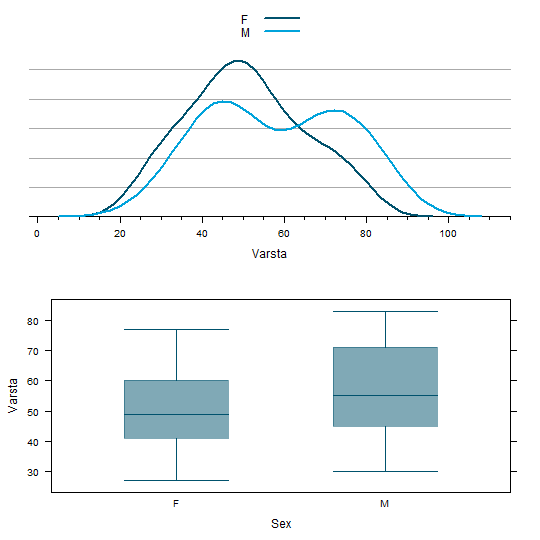
\includegraphics[width=0.8\linewidth]{incoVarstaSex}
   \caption{Distribuția sexelor participanților la studiu}
   \label{fig:Distributia sexelor participantilor la studiu}
  \end{figure}
  %
  Din punct de vedere al greutății am evaluat indicatorul \ac{BMI} conform cu pragurile recomandate de \citep{whobmi06}. 
  Astfel, pentru pacientii de sex feminin avem 13 persoane cu greutate normala ($BMI<25.0$, NOR), 16 supraponderale ($25.0 \geq BMI <30.0$, OVR) și 2 obeze($BMI \geq 30.0$, OBE). 
  Pentru pentru pacientii de sex masculin avem 3 persoane cu greutate normala, 12 supraponderale și 4 obeze.   
  %
  \begin{table}[H]
   \centering
   \begin{tabular}{ |l|l|l|l| }
    \hline
    Sex & NOR & OVR & OBE \\ \hline
    F & 13 & 16 & 2 \\ \hline
    M & 3 &  12 & 4 \\ \hline
   \end{tabular}
   \caption{Numărul de persoane din fiecare categorie \ac{BMI} pe sexe}
   \label{tab:BMIgSex}
  \end{table}
  %
  \begin{figure}[H]
    \centering
    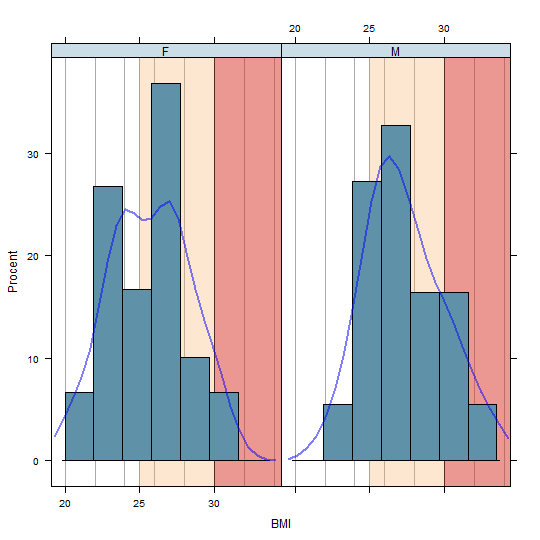
\includegraphics[width=0.8\linewidth]{incobmiDens}
    \caption{Distribuția \ac{BMI} pe sexe, Zona galbena marchează persoanele supraponderale și cea roșie pe cele obeze}
    \label{fig:incobmiDens}
  \end{figure}
  %
  Distribuția \ac{BMI} pe grupa de vârstă și pe sexe a fost evaluată la nivel național conform \citep{EHIS09}, care oferă informații detaliate despre incidenta problemelor de nutriție în rândul tarilor membre ale Uniunii Europene. 
  Din cauza eșantionului foarte mic, nu se poate trage concluzia că populația studiată provine dintr-un eșantion aleator la nivel național dar examinând graficul din Figura~\ref{fig:incoBMIvsEHIS-OOB} se poate observa (cu excepția unor situații particulare - de exemplu toate persoanele de sex masculin din grupa de vârstă 25-44 ani sunt supraponderale sau obeze) că valorile procentelor urmăresc distribuția națională.
  Pentru a testa dacă eșantioanele provin din aceeași distribuție comună am folosit testul \ac{KS} care a dat o probabilitate de 60\% pentru persoanele de sex feminin și de doar 12.4\% pentru persoanele de sex masculin indicând că datele nu sunt suficiente pentru a susține în mod concludent reprezentativitatea eșantionului sau că există un bias de selecție a pacienților în funcție de \ac{BMI}.
  %
  \begin{figure}[H]
    \centering
    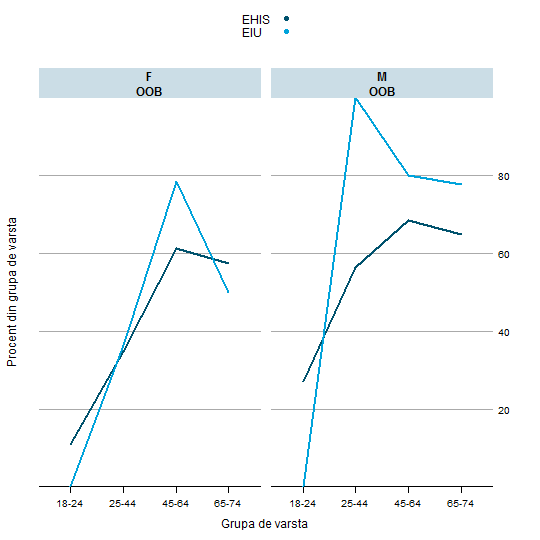
\includegraphics[width=0.8\linewidth]{incoBMIvsEHIS-OOB}
    \caption{Distribuția procentului de persoane obeze în populația studiata (EIU) și în populația generala (EHIS) }
    \label{fig:incoBMIvsEHIS-OOB}
  \end{figure}
  %
  \closeopenmulticols\begin{table}[H]
    \centering
    \begin{tabular}{ |l|l|l|l|l| }
      \hline
      Grupa de vârstă & Sex & Categorie BMI & Număr persoane & Procent \\ \hline
      25-44 & F & NOR & 7  & 63.6 \\ \hline
      25-44 & F & OVR & 3  & 27.3 \\ \hline
      25-44 & F & OBE & 1  &  9.1 \\ \hline
      25-44 & M & NOR & 0  &  0.0 \\ \hline
      25-44 & M & OVR & 4  & 80.0 \\ \hline
      25-44 & M & OBE & 1  & 20.0 \\ \hline
      45-64 & F & NOR & 3  & 21.4 \\ \hline
      45-64 & F & OVR & 10 & 71.4 \\ \hline
      45-64 & F & OBE & 1  &  7.1 \\ \hline
      45-64 & M & NOR & 1  & 20.0 \\ \hline
      45-64 & M & OVR & 3  & 60.0 \\ \hline
      45-64 & M & OBE & 1  & 20.0 \\ \hline
      65-74 & F & NOR & 3  & 50.0 \\ \hline
      65-74 & F & OVR & 3  & 50.0 \\ \hline
      65-74 & F & OBE & 0  &  0.0 \\ \hline
      65-74 & M & NOR & 2  & 22.2 \\ \hline
      65-74 & M & OVR & 5  & 55.6 \\ \hline
      65-74 & M & OBE & 2  & 22.2 \\ \hline
    \end{tabular}
    \caption{Numărul de persoane și procentul din totalul de persoane dintr-o grupa de vârstă din fiecare categorie \ac{BMI} pe sexe și pe grupa de vârstă}
    \label{tab:bmigCounts}
  \end{table}
  %
  
  \begin{multicols}{2}
  Dintre persoanele de sex feminin ($N=31$), 17 sunt la menopauza, 2 paciente au inregistrate cate 3 nasteri, 10 paciente au cate 2 nasteri, 13 paciente au cate o nastere si 6 paciente nu au nici o nastere. Pentru a compara fertilitatea esantionului cu media nationala am calculat indicatorul \ac{ICF} dupa definitia folosita in \citep{insee2011} care a rezultat egal cu $1.125$ fata de media nationala pe anul 2010 de $1.3$ iar rezultatele sub forma grafica sunt afisate in Figura~\ref{fig:incoNasteriICF}.
  %
  \begin{figure}[H]
    \centering
    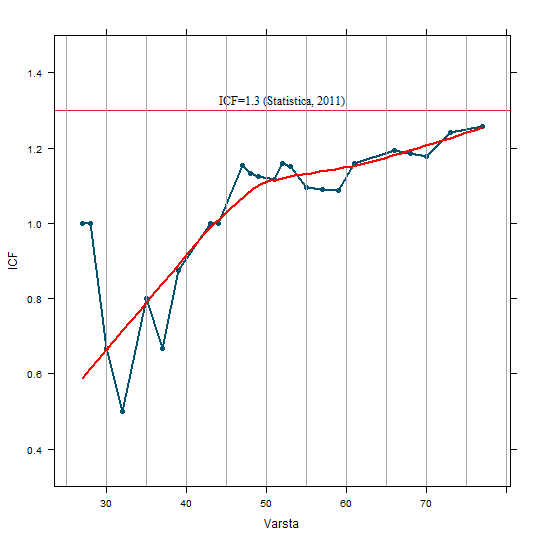
\includegraphics[width=0.8\linewidth]{incoNasteriICF}
    \caption{Variatia ICF cu varsta pacientilor. Se observa convergenta asimptotica catre statistica nationala (linia orizontala rosie) pe masura ce sunt incluse persoanele trecute de perioada fertila }
    \label{fig:incoNasteriICF}
  \end{figure}
  %
  
  Studiul a înregistrat și  date referitor la co-morbiditatea pacientilor colectand date despre prezenta urmatoarelor conditii medicale: bronsita cronica, diabet, sindrom Parkinson, mieilita, spina bifida, depresie, fractura vertebrala, fractura de coloana sau \ac{AVC}. 24 de pacienti nu au raportat nici o conditie Sumarul datelor este prezentat in tabelul \ref{tab:comoSumary}. 
  %
  \begin{table}[H]
    \centering
    \begin{tabular}{ |l|l| }
      \hline
      Conditie medicala & Numar pacienti \\ \hline
      AVC & 7 \\ \hline
      DEPRESIE & 3 \\ \hline
      DIABET & 6 \\ \hline
      FRACTURA COLOANA & 2 \\ \hline
      FRACTURA VERTEBRALA & 1 \\ \hline
      MIELITA & 3 \\ \hline
      PARKINSON & 3 \\ \hline
      SPINA BIFIDA & 1 \\ \hline
    \end{tabular}
    \caption{Conditia medicala si numărul de persoane pentru fiecare}
    \label{tab:comoSumary}
  \end{table}
  %
  Dupa cum se observa in Figura \ref{fig:incoComoCntBySex}, distributia conditiilor medicale variaza foarte mult in functie de sexul pacientului astfel incat pacientii de sex masculin raporteaza cele mai multe cazuri de co-morbiditate ($N_B=17$ vs $N_F=9$) chiar daca numarul lor total este mai mic in esantion ($Total_B=19$ vs $Total_F=31$).
  \begin{figure}[H]
    \centering
    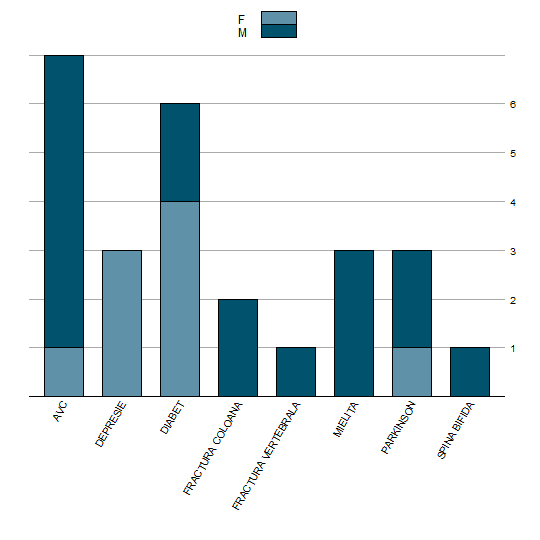
\includegraphics[width=0.8\linewidth]{incoComoCntBySex}
    \caption{Numarul de conditii medicale pentru fiecare sex. }
    \label{fig:incoComoCntBySex}
  \end{figure}
  %

\subsection{Efecte}

  \closeopenmulticols
  
  \bibliographystyle{plainnat}\bibliography{incoStudy}
  
  \section*{Glosar}
  \begin{acronym}[LUTS]
    \acro{IU}{Incontinența Urinară}
    \acro{IUI}{Incontinența Urinară prin Imperiozitate}
    \acro{IUE}{Incontinența Urinară de Efort}
    \acro{IUM}{Incontinența Urinară Mixtă}
    \acro{LUTS}{Lower Urinary Tract Symptoms}
    \acro{SEP}{Stimulare Electrica Periferica}
    \acro{BMI}{Body-Mass Index}
    \acro{KS}{Kolmogorov–Smirnov}
    \acro{ICF}{Indicatorul Conjunctural de Fertilitate}
    \acro{AVC}{Accident vascular cerebral}
    \acro{CEEI}{Chestionar de Evaluare a Impactului Incontinentei}
    \acro{CVDSU}{Calitatea Vietii Datorata Simptomelor Urinare}
    \acro{VAS}{Scala Vizual Analogică pentru evaluarea gradului de îmbunătățire a calității vieții}
    \acro{FEFMP}{Fisa de Evaluare a Fortei Musculaturii Perineale}
    \acro{IGPI}{Impresia Globala a Pacientului de Imbunatatire}
    \acro{USS}{Utilizarea Serviciilor De Sanatate}
  \end{acronym}
 
 \listoffigures
 \listoftables
   
\end{document}
